% !TEX program = pdflatex
% AI-authored internal reference. The student must write the submission independently.
\documentclass[11pt]{article}
\usepackage[margin=0.83in]{geometry}
\usepackage[T1]{fontenc}
\usepackage{lmodern}
\usepackage{microtype}
\usepackage{graphicx}
\usepackage{booktabs}
\usepackage{tabularx}
\usepackage{array}
\usepackage{amsmath,amssymb}
\usepackage{xcolor}
\usepackage{hyperref}
\usepackage{fancyhdr}
\usepackage{caption}
\usepackage{float}
\usepackage{longtable}

\definecolor{navy}{HTML}{173B57}
\definecolor{teal}{HTML}{087E8B}
\definecolor{orange}{HTML}{D95F02}
\definecolor{light}{HTML}{F2F5F7}
\hypersetup{colorlinks=true,linkcolor=navy,urlcolor=teal,citecolor=navy}
\setlength{\parindent}{0pt}
\setlength{\parskip}{0.55em}
\captionsetup{font=small,labelfont=bf}
\pagestyle{fancy}
\setlength{\headheight}{14pt}
\fancyhf{}
\lhead{SEP forecast evaluation audit}
\rhead{Internal reference paper}
\cfoot{\thepage}
\newcommand{\TSS}{\mathrm{TSS}}
\newcommand{\POD}{\mathrm{POD}}
\newcommand{\FPR}{\mathrm{FPR}}
\newcommand{\FAR}{\mathrm{FAR}}
\newcommand{\E}{\mathbb{E}}
\newcommand{\Cov}{\operatorname{Cov}}
\newcommand{\eclass}[1]{\textbf{Evidence class:} #1}

\begin{document}
\pagenumbering{roman}

\begin{titlepage}
\centering
\vspace*{1.3cm}
{\color{navy}\Huge\bfseries What Does a 24-Hour SEP Forecast Score Measure?\par}
\vspace{0.45cm}
{\Large An event-multiplicity and onset-normalized audit of fixed historical forecasts\par}
\vspace{1.1cm}
\rule{0.82\textwidth}{0.8pt}\par
\vspace{0.8cm}
{\large Internal research-reference manuscript\par}
\vspace{0.25cm}
{\large Evidence consolidated 20 September 2026\par}
\vfill
\begin{minipage}{0.88\textwidth}
\colorbox{light}{\parbox{0.94\textwidth}{
\textbf{Authorship and use notice.} This document was generated with AI assistance from a repository audit. It is not eligible to be submitted as the student's initial research paper, abstract, poster, or conclusion. The student must inspect the evidence, read the cited sources, perform and document their own contribution, and write the submission independently. AI-assisted code, analysis, and graphics require accurate disclosure and prompt records under current ISEF guidance.
}}
\end{minipage}
\vfill
{\small Repository audit base: \texttt{13f692a90fc3006181d1c4488da78ff135f24f87}\par
Reference branch head before this manuscript: \texttt{3a9e1842eea9c645665621dac2c481a11f5eb869}}
\end{titlepage}
\clearpage
\pagenumbering{arabic}

\begin{abstract}
Forecasts of solar energetic particle (SEP) conditions are often evaluated at repeated decision times. A multi-day radiation episode can therefore create several positive 24-hour samples, while only its first eligible sample represents prediction of a new onset. This study asks how fixed forecast scores change when the positive sampling unit changes from decision windows to equally weighted physical episodes and then to genuine onset decisions. An immutable historical prediction archive was evaluated without refitting models or altering thresholds. A conservative audit cohort retained only forecast horizons ending strictly before a protected prospective boundary, yielding 7,509 forecast issues, 197 positive windows, 85 represented episodes, and 7,312 negative windows. Joint XGBoost TSS decreased from 0.726 for mapped occurrence to 0.621 for episode-normalized occurrence and 0.437 for onset. The first difference equals an exact multiplicity covariance term, $\Cov(n_i,r_i)/\E[n_i]=0.1053$; the additional episode-to-onset difference is a persistence contribution of 0.1839. A past-proton proxy lost still more onset skill, while a no-proton comparator showed little pooled multiplicity inflation. Paired episode and calendar-cluster bootstrap checks preserved the principal contrast signs, conditional on the frozen forecasts. The result demonstrates that occurrence, episode-normalized, and onset verification answer different operational questions. It does not establish a superior operational model, causal feature effects, or independent prospective performance.
\end{abstract}

\section{Introduction}

Solar energetic particles are high-energy ions, primarily protons, accelerated by solar and interplanetary processes. Operational radiation-storm definitions commonly use integral proton flux above 10 MeV, with 10 particle flux units (pfu) as an important threshold. One pfu denotes one particle per square centimetre per second per steradian. Such storms can affect astronauts, spacecraft electronics, communications, and polar aviation operations \cite{whitman2023,sepprism2026}.

Forecast verification depends on the decision being evaluated. A forecast that recognizes radiation exposure already in progress may be useful for maintaining protective actions. A forecast that warns of a genuinely new onset supports a different decision. These are both legitimate targets, but their scores should not be interpreted as interchangeable.

The audited SEP-PRISM table uses fixed, non-overlapping 24-hour predictor windows paired with subsequent 24-hour targets \cite{sepprism2026}. Repetition in this study is therefore not caused by overlapping input windows. It arises because one multi-day physical episode can intersect several successive target windows. If longer episodes are easier to recognize, a randomly selected positive window overrepresents those episodes and can produce a different sensitivity from a uniformly selected physical episode.

The research question is:

\begin{quote}
For the same frozen forecast probabilities and thresholds, how do forecast skill and interpretation change when evaluation moves from mapped occurrence windows, to equal weighting of represented SEP episodes, to genuine new-onset decisions?
\end{quote}

The contribution is an empirical estimand audit, an exact attribution of the sensitivity difference, matched negative-cohort comparisons, and explicit preservation of negative forecasting and data-source results. The covariance identity itself is established reweighting mathematics related to informative cluster size and size-biased sampling \cite{nevalainen2014,frank2012}; it is not claimed as a new theorem.

\section{Data, forecasts, and evidence boundaries}

\subsection{Source data and target semantics}

The source table was traced to \texttt{yuyian/SEP-Prediction-V2} revision \texttt{e138dcd72c19}; the complete 40-character revision is recorded in the evidence manifest. The full released table contains 14,464 daily windows and 650 positive operational-SEP windows. A frozen model-free audit reported 614 uniquely mapped positive windows representing 257 catalog episodes, an episode-multiplicity factor of 2.389. It classified 418 as already-active or persistence windows, 228 as onset windows, four as ambiguous positives, and 36 as multi-event overlaps in a separate mapping category.

These counts establish agreement with the declared catalog mapping. They do not independently reconstruct event intervals from raw proton-flux measurements, and the term ``physical episode'' remains conditional on the catalog definition.

\subsection{Frozen prediction design}

The principal benchmark used expanding chronological roles:

\begin{itemize}
\item fit 1986--1999, threshold 2000--2004, score 2005--2010;
\item fit 1986--2004, threshold 2005--2010, score 2011--2017;
\item fit 1986--2010, threshold 2011--2017, score 2018--the original endpoint.
\end{itemize}

The archived benchmark contains joint and no-proton XGBoost ensembles, joint and no-proton elastic-net controls, a past-proton threshold proxy, and fit-prevalence climatology. Thresholds were chosen on threshold roles using the declared TSS rule. The evaluation audit reads immutable issue-level predictions and stored thresholds; it does not refit models.

Chronological separation does not make these results independent confirmation because the public data and earlier diagnostics were development-exposed. Retrospective harmonization and interpolation also do not prove that every feature was causally available at its historical issue time.

\subsection{Protected-boundary guard}

Repository contracts disagree about the prospective boundary. The newest contract protects outcomes from 2025-09-10 00:00 UTC inclusively, while older wording used a different convention. The audit therefore admits a row only when its issue time plus 24 hours is strictly earlier than the protected boundary. Timestamp selection occurs before outcome, probability, or episode fields are interpreted for excluded rows. No excluded outcome counts or event identities are emitted.

The resulting independently recomputed historical diagnostic contains 7,509 issues, 197 positive windows, 85 represented episodes, 112 already-active positive windows, 7,312 negatives, and 1,080 quiet blocks. This is a new, explicitly labeled diagnostic subset. It does not replace the original frozen endpoint.

\section{Evaluation estimands and metrics}

Three positive-population views were applied to identical probabilities and thresholds:

\begin{enumerate}
\item \textbf{Mapped occurrence}: each admitted positive decision window has equal weight.
\item \textbf{Episode-normalized occurrence}: each represented episode has total weight one, distributed uniformly across its positive windows.
\item \textbf{New onset}: only the single eligible onset window from each represented episode remains positive.
\end{enumerate}

Negative rows and their weights are identical across the three primary views. Thus the false-positive rate cancels in within-model TSS contrasts. Episode-normalized sensitivity is the mean fraction of positive windows alerted within an episode; it is not the fraction of episodes alerted at least once.

For weighted confusion-matrix masses,
\begin{align}
\POD &= \frac{TP}{TP+FN}, &
\FPR &= \frac{FP}{FP+TN},\\
\FAR &= \frac{FP}{TP+FP}, &
\TSS &= \POD-\FPR.
\end{align}
HSS and Brier score were also computed. FAR answers ``what fraction of issued alerts were false?'' while FPR answers ``what fraction of negative decisions were alerted?'' They must not be interchanged.

\section{Exact multiplicity and persistence mechanism}

Let $K$ represented positive episodes have multiplicity $n_i>0$. Let $a_{ij}\in\{0,1\}$ be the fixed alert for positive window $j$ of episode $i$, and let
\[
r_i=\frac{1}{n_i}\sum_{j=1}^{n_i}a_{ij}.
\]
Under the uniform distribution over represented episodes,
\[
\POD_{\rm row}=\frac{\E[nr]}{\E[n]},\qquad
\POD_{\rm episode}=\E[r].
\]
Since $\E[nr]=\E[n]\E[r]+\Cov(n,r)$,
\begin{equation}
\boxed{\POD_{\rm row}-\POD_{\rm episode}
=\frac{\Cov(n,r)}{\E[n]}.}
\label{eq:cov}
\end{equation}

The covariance is a finite-population covariance with denominator $K$. Equation~\ref{eq:cov} is exact and requires no independence assumption. The gap is zero if and only if the covariance is zero; statistical independence is sufficient but unnecessary. For TSS, the same identity holds only when the negative measure is unchanged. Otherwise, one must add $\FPR_{\rm episode}-\FPR_{\rm row}$.

Assume each admitted episode contains exactly one onset alert indicator $u_i$ and $n_i-1$ active-window alerts whose mean is $v_i$. Then
\[
r_i=\frac{u_i}{n_i}+\left(1-\frac{1}{n_i}\right)v_i,
\]
so that
\begin{equation}
\boxed{
\TSS_{\rm row}-\TSS_{\rm onset}
=\frac{\Cov(n,r)}{\E[n]}
+\E\!\left[\left(1-\frac{1}{n}\right)(v-u)\right]
}
\label{eq:persistence}
\end{equation}
for the matched negative cohort. The first term quantifies multiplicity reweighting; the second compares within-episode active-window and onset detection. This is an algebraic attribution, not proof that a proton feature causally produces the difference.

More generally, reweighting any base distribution $b_i$ by nonnegative $w_i$ yields
\[
\E_{bw}[r]-\E_b[r]=\frac{\Cov_b(w,r)}{\E_b[w]}.
\]
This connects row sampling to size-biased sampling and episode normalization to inverse-cluster weighting. A useful bound is
\[
|\POD_{\rm row}-\POD_{\rm episode}|
\leq \mathrm{CV}(n)\,\mathrm{SD}(r)\leq \frac{\mathrm{CV}(n)}{2}.
\]
Greater multiplicity variation permits a larger difference but does not force one.

\section{Results}

\subsection{Primary fixed-prediction comparison}

\begin{table}[H]
\centering
\caption{TSS for identical frozen forecasts under three estimands in the strict historical diagnostic.}
\label{tab:tss}
\begin{tabular}{lrrr}
\toprule
Model & Mapped occurrence & Episode-normalized & New onset\\
\midrule
Joint XGBoost & 0.726442 & 0.621115 & 0.437222\\
No-proton XGBoost & 0.509010 & 0.514845 & 0.477478\\
Past-proton proxy & 0.601221 & 0.446980 & 0.092890\\
Joint elastic net & -0.122857 & -0.182905 & -0.267079\\
No-proton elastic net & -0.319035 & -0.332204 & -0.333128\\
Fit-prevalence climatology & 0 & 0 & 0\\
\bottomrule
\end{tabular}
\end{table}

The joint XGBoost headline changes materially as the question changes. Its mapped-to-episode reduction is 0.105327 and its episode-to-onset reduction is 0.183894. Together they exactly reproduce the mapped-to-onset difference of 0.289221, with numerical residual below $10^{-16}$. For this model the row sensitivity is 0.7716, episode-average window sensitivity is 0.6662, onset sensitivity is 0.4824, and at-least-once episode detection is 0.8000. These are distinct quantities.

The past-proton proxy loses 0.508331 TSS from mapped occurrence to onset, consistent with strong recognition of recent/continuing proton activity. The no-proton XGBoost pooled multiplicity contribution is -0.005835 and its persistence contribution is 0.037367. This is a useful comparator, but it does not prove causal independence; its behavior varies across temporal folds.

\begin{figure}[H]
\centering
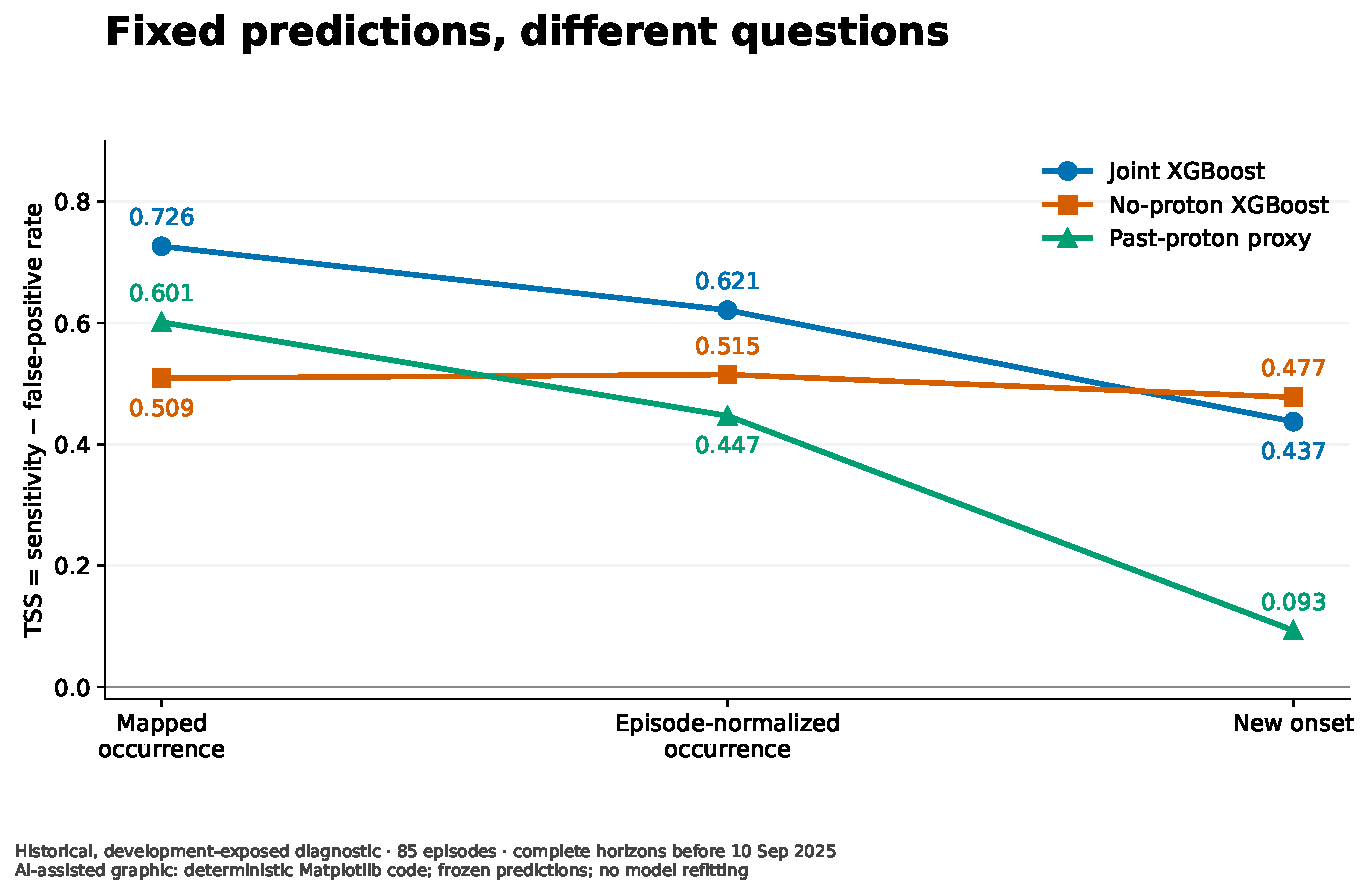
\includegraphics[width=0.94\textwidth]{../audit_20260915/figures/01_fixed_predictions.pdf}
\caption{The same frozen alerts answer different questions under different positive sampling units. Lines indicate changes in evaluation, not training trajectories. Historical and development-exposed evidence.}
\end{figure}

\subsection{Confusion matrices and alert burden}

\begin{table}[H]
\centering
\caption{Strict historical diagnostic for the three principal comparators. Episode-normalized TP and FN are weighted masses.}
\small
\begin{tabular}{llrrrrrr}
\toprule
Model & View & TP & FN & FP & TN & POD & FAR\\
\midrule
Joint & Mapped & 152.000 & 45.000 & 330 & 6982 & 0.7716 & 0.6846\\
Joint & Episode & 56.631 & 28.369 & 330 & 6982 & 0.6662 & 0.8535\\
Joint & Onset & 41.000 & 44.000 & 330 & 6982 & 0.4824 & 0.8895\\
No proton & Mapped & 136.000 & 61.000 & 1326 & 5986 & 0.6904 & 0.9070\\
No proton & Episode & 59.176 & 25.824 & 1326 & 5986 & 0.6962 & 0.9573\\
No proton & Onset & 56.000 & 29.000 & 1326 & 5986 & 0.6588 & 0.9595\\
Past-proton proxy & Mapped & 121.000 & 76.000 & 95 & 7217 & 0.6142 & 0.4398\\
Past-proton proxy & Episode & 39.098 & 45.902 & 95 & 7217 & 0.4600 & 0.7084\\
Past-proton proxy & Onset & 9.000 & 76.000 & 95 & 7217 & 0.1059 & 0.9135\\
\bottomrule
\end{tabular}
\end{table}

The joint model's onset FPR is 0.0451, but its onset FAR is 0.8895. This means relatively few negative decisions are alerted, yet most alerts are false because onsets are rare. That distinction is operationally important: a low FPR alone does not imply a manageable alert stream.

\subsection{Mechanism estimates}

\begin{table}[H]
\centering
\caption{Exact decomposition of mapped-minus-onset TSS.}
\begin{tabular}{lrrr}
\toprule
Model & Multiplicity & Persistence & Total difference\\
\midrule
Joint XGBoost & 0.105327 & 0.183894 & 0.289221\\
No-proton XGBoost & -0.005835 & 0.037367 & 0.031532\\
Past-proton proxy & 0.154241 & 0.354090 & 0.508331\\
Joint elastic net & 0.060048 & 0.084174 & 0.144222\\
No-proton elastic net & 0.013169 & 0.000924 & 0.014094\\
\bottomrule
\end{tabular}
\end{table}

\begin{figure}[H]
\centering
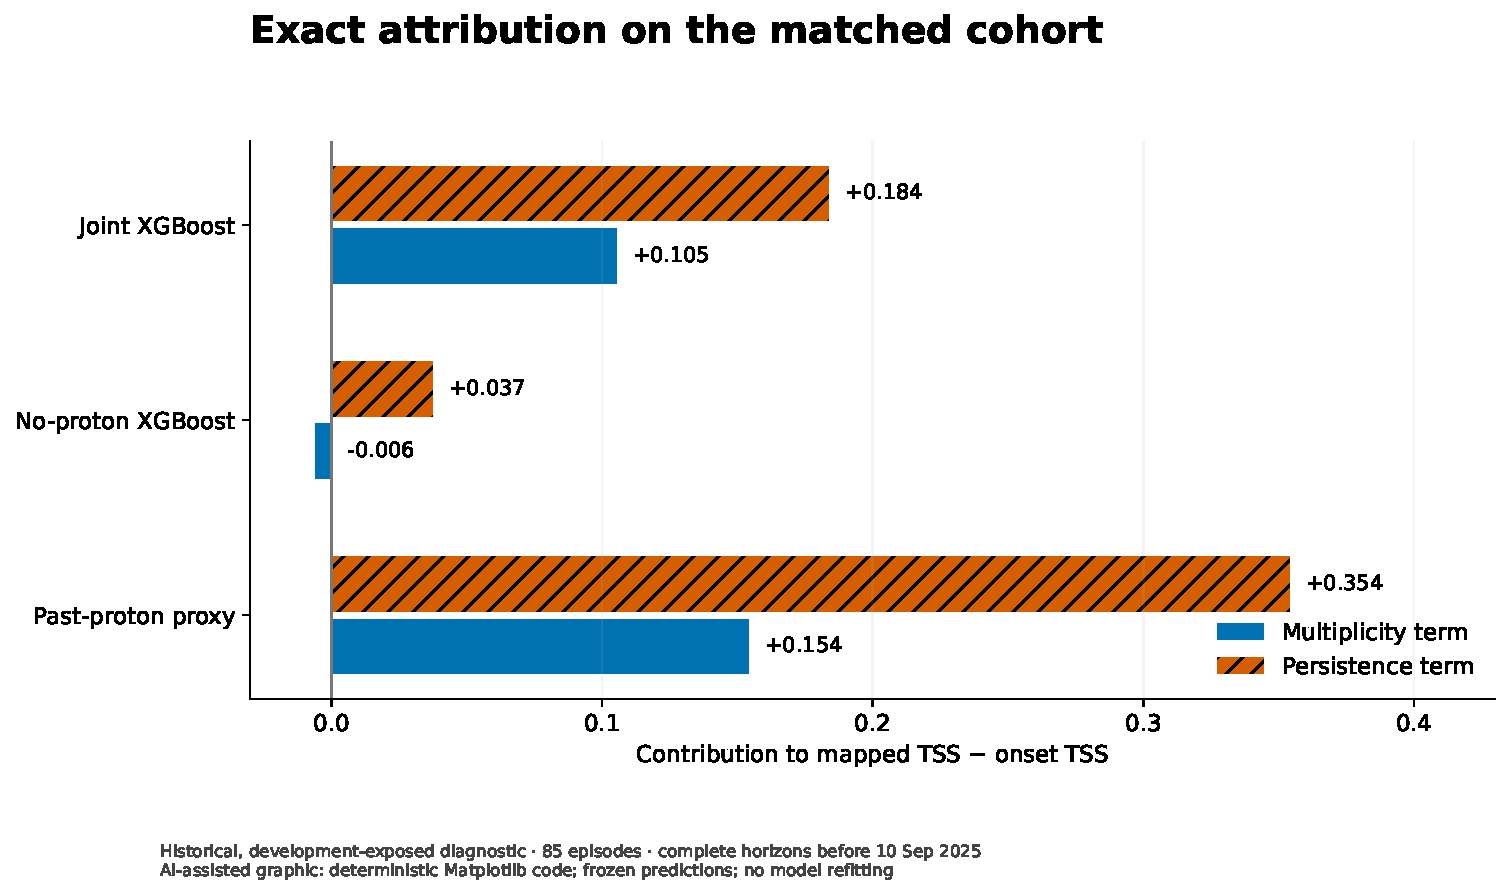
\includegraphics[width=0.94\textwidth]{../audit_20260915/figures/02_decomposition.pdf}
\caption{Multiplicity and persistence contributions for three comparators. Negative contributions are possible. The decomposition is exact on the declared matched cohort.}
\end{figure}

\subsection{Uncertainty and temporal clustering}

The new paired bootstrap used 10,000 shared draws (seed 20260915), sampling positive episodes and negative quiet blocks as clusters. The joint normalized-minus-mapped contrast had a 95\% percentile interval of $[-0.1469,-0.0637]$. The joint onset-minus-normalized contrast had interval $[-0.2454,-0.1251]$. The proxy onset-minus-mapped interval was $[-0.5676,-0.4417]$. The paired joint-minus-no-proton onset interval, $[-0.1641,0.0838]$, includes zero; therefore a reliable onset rank reversal is not demonstrated.

Nearby episodes can share solar-cycle and active-region conditions. An additional post-hoc check resampled complete 27-day, 90-day, quarterly, and yearly calendar bins, including empty bins. Across all four choices, the 95\% intervals for the joint multiplicity and persistence contrasts remained negative. The yearly intervals were approximately $[-0.1538,-0.0584]$ and $[-0.2456,-0.1175]$. These checks support the sign of the historical contrasts but do not establish stationarity, account for the full model-selection process, or create prospective validation.

\begin{figure}[H]
\centering
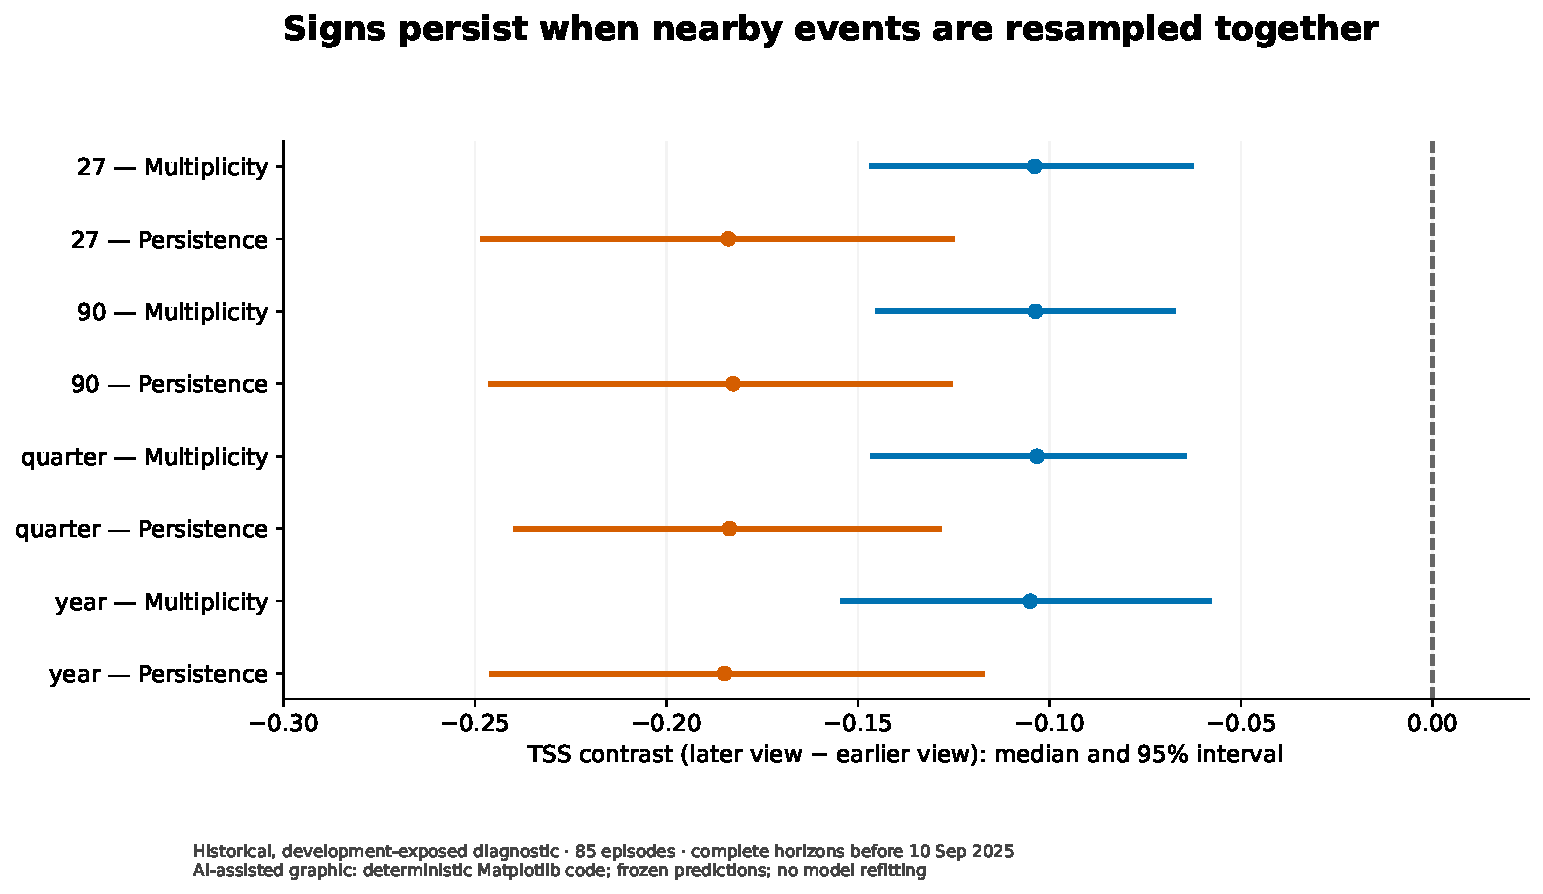
\includegraphics[width=0.94\textwidth]{../audit_20260915/figures/03_temporal_intervals.pdf}
\caption{Paired temporal-cluster bootstrap medians and 95\% intervals for the joint model. All are conditional on frozen forecasts. The fraction of bootstrap draws with one sign is not a null-hypothesis $p$-value.}
\end{figure}

\subsection{Secondary metrics}

For joint XGBoost, mapped/episode/onset HSS values are 0.4264, 0.2256, and 0.1642. Corresponding Brier scores are 0.01387, 0.00850, and 0.01139. These values cannot be read as a simple improvement sequence because episode reweighting changes the class prevalence. The observed row-to-episode Brier difference decomposes into a positive-row loss reweighting term of -0.003526 and a prior-shift term of 0.008901. Joint occurrence AUROC changes from 0.9445 under row weighting to 0.9173 under episode weighting when the negative distribution is fixed.

\section{Negative and non-confirmatory results}

Negative results constrain the claims and are part of the contribution.

\begin{longtable}{p{0.20\textwidth}p{0.44\textwidth}p{0.28\textwidth}}
\caption{Major unsuccessful or non-confirmatory experiments.}\\
\toprule
Study & Result & Disposition\\
\midrule
\endfirsthead
\toprule
Study & Result & Disposition\\
\midrule
\endhead
Elastic-net controls & Negative TSS in all three views for both feature sets. & Retain; no useful absolute forecast skill.\\
Direct Phase II & One score-period onset. Engineered TSS 0.488 versus baseline 0.411; improvement interval includes zero. & Underpowered, development-exposed.\\
Separate Phase-II PR & 3,219 rows and 21 positives. Selected method TSS 0.168 versus regular 0.366; difference $-0.198$ with interval spanning zero. & Promotion criterion failed.\\
Controller V1 & TP 0, FN 1, FP 41, TN 168; TSS $-0.196$. & Lower FPR missed the only onset.\\
Controller V2 & TP 1, FN 0, FP 50, TN 159; TSS 0.761, FPR 23.9\%, FAR 98.0\%. & Post-hoc, one-event result; not validated.\\
NOAA SGPS L2 & Historical differential products did not satisfy the presumed live integral-channel contract. & No operational model trained.\\
L1b mapping & Telescope/channel arrays were not bound to the live 13-channel predictor semantics. & Fail closed; impossibility not proved.\\
NSRRD science L2 & Coverage and energy proximity were insufficient; both yaw-state sensor reductions were not verified. & Reprocessed science data cannot be called operational.\\
Alert recovery & An uncommitted local report states that all candidates failed advancement; reduced outage false alerts required additional missed onsets. & Unverified development evidence, excluded from central claims.\\
\bottomrule
\end{longtable}

\section{Practical usefulness}

The project is useful, but its usefulness is primarily methodological and decision-supporting rather than a deployed warning system.

\subsection{For space agencies and forecast centres}

The study supplies a verification template that prevents one headline number from answering several incompatible questions. A forecast centre can report:

\begin{itemize}
\item decision-window performance for maintaining precautions during continuing exposure;
\item episode-normalized performance so long events do not dominate comparisons;
\item onset-only performance for issuing new warnings;
\item alert burden through both FPR and FAR;
\item lead-time and source-availability evidence when those data are genuinely causal.
\end{itemize}

This can change model procurement and validation decisions. A model that is effective at recognizing already-active storms may be suitable for exposure-state awareness but poor for advance warning. Conversely, a model with lower occurrence TSS may still be more useful for onset if it performs at an acceptable alert burden. The audit makes those trade-offs inspectable.

\subsection{For companies}

Satellite operators, launch providers, aviation stakeholders, and mission-planning teams need different decisions: enter or maintain a safe mode, reschedule activity, increase monitoring, or do nothing. A three-estimand verification card helps them ask vendors for evidence aligned with the intended action. The present study does not quantify monetary savings, avoided damage, or operator adoption. Those benefits remain plausible use cases requiring a cost model and prospective operational testing.

\subsection{For SEP researchers}

The exact covariance term turns a qualitative concern about repeated events into a measurable diagnostic. It also identifies when row and episode metrics agree: precisely when episode multiplicity and within-episode detectability have zero covariance under the declared population. This supports more transparent cross-model comparisons and exposes rank changes caused by estimand choice rather than retraining.

\section{Discussion}

The strongest scientific finding is not that conventional occurrence scoring is wrong. Occurrence scoring is appropriate when every future decision interval represents a real operational exposure decision. The finding is that occurrence, equal-event, and onset evaluation estimate different quantities. Reporting only one can invite an interpretation that the experiment did not test.

The joint model's strong mapped TSS reflects both genuine predictive discrimination and the weighting of detectable multi-window episodes. Removing multiplicity reduces TSS by about 0.105; isolating onsets reduces it by another 0.184. The past-proton proxy provides a falsification-oriented control: it performs reasonably on mapped occurrence and very poorly on onset, as expected for a rule tied to recent proton activity. The no-proton comparator's small pooled multiplicity term shows that a large gap is not mathematically inevitable, although its high false-alert burden prevents it from being promoted as a better operational system.

The exact identity is related to established work on informative cluster size and changes of measure \cite{nevalainen2014,frank2012}. Event-based forecast verification is also established in solar forecasting \cite{kso2018}. The defensible novelty claim is narrower: a fixed-prediction SEP application that combines decision-window, equal-episode, and onset estimands; exact attribution; paired clustered uncertainty; controls; and an immutable evidence trail. A bounded search did not establish universal priority, so ``first'' and ``new theorem'' claims are not supported.

\section{Limitations}

\begin{enumerate}
\item \textbf{Development exposure.} The historical data and several diagnostics were previously inspected. The result is mechanistic historical evidence, not independent confirmation.
\item \textbf{Event semantics.} Episodes are defined by a catalog. Alternative predeclared event merging, onset, and threshold rules could change multiplicities and cohort membership.
\item \textbf{Causal availability.} Retrospective harmonized predictors may not have been available with the same latency and quality at issue time.
\item \textbf{Protected boundary.} Conflicting repository wording blocks unrestricted full-endpoint replay. The audit uses a conservative strict-horizon subset and leaves protected outcomes sealed.
\item \textbf{Conditional uncertainty.} Bootstrap intervals condition on fitted models, thresholds, event definitions, and the fixed archive. They exclude full model-selection and source-construction uncertainty.
\item \textbf{Rare onsets.} Eighty-five historical episodes support the central estimand audit, but one-event Phase-II and controller experiments cannot validate operational performance.
\item \textbf{Impact not measured.} The project proposes a useful verification practice; it has not demonstrated reduced spacecraft loss, cost savings, or operator adoption.
\item \textbf{Student ownership and compliance.} Competition eligibility depends on documented current-year student work, proper AI disclosure, approvals, and an unaided expert defense. This reference manuscript does not provide that evidence.
\end{enumerate}

\section{Falsification and future work}

The project should be weakened or revised if a predeclared alternative physical-event definition removes the principal contrast; if genuinely preissued, sealed prospective forecasts show similar occurrence and onset behavior; if causal live-source reconstruction invalidates the historical feature interpretation; or if literature review finds the same complete SEP design and attribution already established.

The highest-value future experiment is not another retrospective threshold search. It is an independently custodied prospective study with predictions timestamped before outcomes, a verified live-source contract, enough new onset episodes and quiet blocks, fixed endpoints, and paired analysis specified in advance. Operational work should additionally evaluate warning lead time, alert duration, abstentions, source failures, and decision-specific costs.

\section{Competition assessment}

\subsection{Can this project win?}

It can be competitive and could win an award, but a win is not predictable or guaranteed. The project has a clear question, a reproducible design, nontrivial statistics, an exact mechanism, preserved negative results, and potential impact on how SEP models are compared. These map well to research question, methodology, execution, creativity, and impact criteria. Current ISEF judging places 35 of 100 points on presentation, including 25 for the interview \cite{isefcriteria2026}; student understanding and independence are therefore decisive.

Its largest competitive liabilities are also real: the data were development-exposed, the mathematics is an application of known reweighting ideas, operational causality is unresolved, and the work may look like ``only evaluation'' unless the student can explain the concrete decision consequences. A judge may also reject exaggerated novelty, an operational forecasting claim, or weak evidence of student ownership.

The most truthful assessment is:

\begin{itemize}
\item \textbf{Useful? Yes.} It identifies a consequential mismatch between forecast score interpretation and operational question, and supplies a reproducible way to measure it.
\item \textbf{Scientifically defensible? Yes, within the historical conditional scope stated here.}
\item \textbf{A proven forecasting breakthrough? No.}
\item \textbf{Capable of winning? Yes, if the student owns the reasoning, writes independently, survives technical questioning, and keeps claims narrow.}
\item \textbf{Likely to win automatically because the numbers look strong? No.} Judging quality, competing projects, eligibility, originality evidence, and interview performance are unknown.
\end{itemize}

The strongest presentation is a transparent methodological discovery with practical consequences, not a claim to have solved SEP forecasting.

\section{Reproducibility and evidence classification}

The audit code pins source-archive hashes, validates stored alerts against probabilities and thresholds, refuses protected-boundary horizons, and writes to new output directories. Fifty-one selected scientific tests passed on 20 September 2026. Three principal aggregate outputs reproduced byte-for-byte in the prior audit. Generated technical figures are explicitly labeled AI-assisted.

Claims should retain these evidence classes:

\begin{description}
\item[Level A:] directly demonstrated by immutable or independently recomputed historical evidence.
\item[Level B:] mathematically derived from Level-A quantities under stated assumptions.
\item[Level C:] supported but exploratory or post-hoc.
\item[Level D:] hypothesis, proposed use, or future study.
\item[Level X:] unsupported and removed from the paper claim set.
\end{description}

Central score changes are Level A; the exact decompositions are Level B; calendar-cluster robustness and application novelty are Level C; operational benefit and prospective generalization are Level D. Claims of a new theorem, validated controller TSS 0.76, universal score inflation, state-of-the-art performance, or operational readiness are Level X.

\section{Conclusion}

Fixed 24-hour SEP forecasts can receive materially different scores depending on whether evaluation samples positive decision windows, equally weighted represented episodes, or genuine new onsets. In the audited historical cohort, joint-model TSS declined from 0.726 to 0.621 to 0.437 across those views. The first change is exactly explained by covariance between episode multiplicity and detectability, and the second by the relative detection of active versus onset windows. The result supports routine multi-estimand reporting for SEP forecast evaluation. It does not establish an independently validated onset forecaster. Its value lies in clarifying what a score rewards, aligning evidence with operational decisions, and making limitations difficult to hide.

\section*{Data and code availability}

The repository evidence package is located under \texttt{iris\_report/iris\_sep/audit\_20260915/}. The consolidated evidence file is \texttt{PAPER\_RESULTS\_20260920.md}. Immutable archives are referenced by SHA-256 in \texttt{archive\_manifest.json}; archives containing protected-boundary records are intentionally excluded from distributable bundles. Draft pull request 7 contains the audit branch for review. No protected prospective outcomes were scored for this manuscript.

\section*{AI and contributor disclosure}

This reference manuscript, audit code, selected analyses, and technical figures received generative-AI assistance. The student must not represent this manuscript as their independently authored initial submission. Student, mentor, custodian, software, and AI contributions must be recorded accurately. Current ISEF rules require integrity, presentation in the student's own words, and evaluation of the finalist's independence and understanding \cite{isefrules2026,isefcriteria2026}.

\begin{thebibliography}{99}

\bibitem{sepprism2026}
Y. Yu et al., ``SEP-PRISM Data: A multi-source dataset for solar energetic particle forecasting,'' arXiv:2607.16160, 2026. \url{https://arxiv.org/abs/2607.16160}

\bibitem{sepnetprism2026}
Y. Yu et al., ``SEPNET-PRISM Model,'' arXiv:2606.14440, 2026. \url{https://arxiv.org/abs/2606.14440}

\bibitem{sepnet2026}
Y. Yu et al., ``Solar Energetic Particle Forecasting with Multi-Task Deep Learning: SEPNet,'' arXiv:2512.12786. \url{https://arxiv.org/abs/2512.12786}

\bibitem{whitman2023}
K. Whitman et al., ``Review of solar energetic particle prediction models,'' \emph{Advances in Space Research}, vol. 72, pp. 5161--5242, 2023, doi:10.1016/j.asr.2022.08.006.

\bibitem{nevalainen2014}
J. Nevalainen, S. Datta, and H. Oja, ``Inference on the marginal distribution of clustered data with informative cluster size,'' \emph{Statistical Papers}, vol. 55, pp. 71--92, 2014, doi:10.1007/s00362-013-0504-3.

\bibitem{frank2012}
S. A. Frank, ``Natural selection. IV. The Price equation,'' \emph{Journal of Evolutionary Biology}, vol. 25, pp. 1002--1019, 2012, doi:10.1111/j.1420-9101.2012.02498.x.

\bibitem{kso2018}
A. Veronig et al., ``An event-based verification scheme for a real-time flare detection system at Kanzelhöhe Observatory,'' \emph{Solar Physics}, vol. 293, article 94, 2018, doi:10.1007/s11207-018-1312-7.

\bibitem{aspecs2022}
European Space Agency, ``Forecasting Solar Storms with the Solar Energetic Particle Advanced Warning System,'' ASPECS technical study, 2022. \url{https://nebula.esa.int/sites/default/files/neb_tec_studies/2775/public/4000120480_EX.pdf}

\bibitem{noaaverification}
NOAA Space Weather Prediction Center, ``Forecast Verification.'' \url{https://www.spaceweather.gov/content/forecast-verification}

\bibitem{isefcriteria2026}
Society for Science, ``Regeneron ISEF Grand Award Judging Criteria,'' accessed 20 September 2026. \url{https://www.societyforscience.org/isef/grand-award/criteria/}

\bibitem{isefrules2026}
Society for Science, ``Regeneron ISEF Rules for All Projects,'' accessed 20 September 2026. \url{https://www.societyforscience.org/isef/international-rules/rules-for-all-projects/}

\end{thebibliography}

\appendix
\section{Compact result ledger}

\begin{table}[H]
\centering
\caption{Joint XGBoost strict-diagnostic metrics.}
\begin{tabular}{lrrrrrr}
\toprule
View & POD & FPR & FAR & TSS & HSS & Brier\\
\midrule
Mapped & 0.7716 & 0.0451 & 0.6846 & 0.7264 & 0.4264 & 0.01387\\
Episode normalized & 0.6662 & 0.0451 & 0.8535 & 0.6211 & 0.2256 & 0.00850\\
New onset & 0.4824 & 0.0451 & 0.8895 & 0.4372 & 0.1642 & 0.01139\\
\bottomrule
\end{tabular}
\end{table}

\begin{table}[H]
\centering
\caption{Principal paired bootstrap contrasts, strict historical diagnostic.}
\begin{tabular}{lrrr}
\toprule
Contrast & Point & Bootstrap median & 95\% interval\\
\midrule
Joint: episode $-$ mapped & -0.1053 & -0.1040 & [-0.1469, -0.0637]\\
Joint: onset $-$ episode & -0.1839 & -0.1832 & [-0.2454, -0.1251]\\
Proxy: onset $-$ mapped & -0.5083 & -0.5069 & [-0.5676, -0.4417]\\
Joint $-$ no proton, onset & -0.0403 & -0.0407 & [-0.1641, 0.0838]\\
\bottomrule
\end{tabular}
\end{table}

\section{Terms a judge may test}

\begin{description}
\item[10 MeV:] particle kinetic-energy threshold for an integral proton channel, not a flux.
\item[10 pfu:] operational flux threshold; one pfu is one particle cm$^{-2}$ s$^{-1}$ sr$^{-1}$.
\item[Onset:] first eligible forecast decision associated with the beginning of a catalog episode under the declared mapping.
\item[Persistence:] a positive target window after the episode has already begun.
\item[Informative cluster size:] cluster size is associated with the outcome or statistic of interest, so random-row and random-cluster estimands differ.
\item[Paired bootstrap:] both sides of a contrast use the same sampled physical units, preserving covariance and reducing irrelevant variability.
\item[Prospective:] prediction fixed and recorded before its outcome, under a causally available source contract; a later freeze of historical predictions is not prospective.
\end{description}

\end{document}
